\documentclass[hyperref=unicode]{beamer}

\usepackage[absolute,overlay]{textpos}
\usepackage{graphicx}
\usepackage{adjustbox}
\usepackage{chemfig}
\usepackage[version=4]{mhchem}
\usepackage{wrapfig}
\usepackage{multirow}
\adjustboxset*{center}
\usepackage{caption}
\usepackage{chemformula}
\usepackage{elements}

%dělení slov
\usepackage{ragged2e}
\let\raggedright=\RaggedRight
%konec dělení slov

\usepackage{fontspec}
\usepackage{unicode-math}

\usepackage{polyglossia}
\setdefaultlanguage{czech}

\def\uv#1{„#1“}

\mode<presentation>{\usetheme{Madrid}}
\DefineNamedColor{named}{pozadi}{RGB}{200,200,200}
\usecolortheme{crane}

\setbeamertemplate{footline}[frame number]

\addtobeamertemplate{frametitle}{
	\let\insertframetitle\insertsectionhead}{}
\addtobeamertemplate{frametitle}{
	\let\insertframesubtitle\insertsubsectionhead}{}

\makeatletter
\CheckCommand*\beamer@checkframetitle{\@ifnextchar\bgroup\beamer@inlineframetitle{}}
\renewcommand*\beamer@checkframetitle{\global\let\beamer@frametitle\relax\@ifnextchar\bgroup\beamer@inlineframetitle{}}
\makeatother
\setbeamercolor{section in toc}{fg=blue}
\setbeamertemplate{section in toc shaded}[default][100]

\title[Crisis]
{Plyny}

\subtitle{Ideální plyn, stavová rovnice, plynové zákony}

%\author{Zdeněk Moravec, \href{http://z-moravec.net/chemie/zaklady-chemie/}{http://z-moravec.net}}
\author{Zdeněk Moravec, hugo@chemi.muni.cz}

\date{}
\begin{document}

	\frame{\titlepage}

\section{Ideální plyn}
\frame{
  \frametitle{}
  \vfill
\begin{itemize}
  \item Částice plynu lze považovat za hmotné body, tzn. plyn lze stlačit na nulový objem, ale nelze jej zkapalnit
  \item Částice spolu neinteragují, pouze se srážejí
  \item Částice se při srážkách chovají jako dokonale pružná tělesa, tzn. nevyměňují si energii
  \item 1 mol ideálního plynu má objem 22,414 dm$^3$ \\ (molární objem $V_m$)
  \item $n=\frac{V}{V_m}$ [mol]
\end{itemize}

\begin{center}
\begin{tabular}{|c|r@{,}l|}
\hline
\textbf{Plyn} & \multicolumn{2}{|c|}{\textbf{Objem 1 molu plynu [$dm^3$]}} \\
\hline
Ideální plyn & 22 & 414 \\\hline
Ar & 22 & 09 \\\hline
CO$_2$ & 22 & 26 \\\hline
N$_2$ & 22 & 40 \\\hline
O$_2$ & 22 & 40 \\\hline
H$_2$ & 22 & 43 \\\hline
\end{tabular}
\end{center}
  \vfill
}

\section{Standardní podmínky}
\frame{
	\frametitle{}
	\begin{itemize}
		\item IUPAC definuje standardní podmínky pro plyny:\footnote[frame]{\href{https://goldbook.iupac.org/terms/view/S05910}{standard conditions for gases}}
		\begin{itemize}
			\item Teplota: 273,15 K (0~$^\circ$C)
			\item Tlak: 10$^5$~Pa = 100~kPa
		\end{itemize}
		\item Dříve používaný standardní tlak 1 atmosféry, tj. 101 325 Pa je už zastaralý.
	\end{itemize}
}

\section{Stavová rovnice}
\frame{
 \frametitle{}
\begin{columns}
\column{.5\textwidth}
\begin{itemize}
  \item $p.V = nRT = \frac{m}{MRT}$
  \item $\rho = \frac{pM}{RT}$
  \item $M = \frac{\rho RT}{p} = \frac{RT}{V_m}$
  \item \small R = 8,314 4621(75) J.K$^{-1}$.mol$^{-1}$; molární plynová konstanta
  \item Pro změny stavu plynu platí:
  \item \scalebox{1.3}{$\frac{p_1V_1}{n_1T_1} = \frac{p_2V_2}{n_2T_2}$}
\end{itemize}

\column{.5\textwidth}
\begin{figure}
	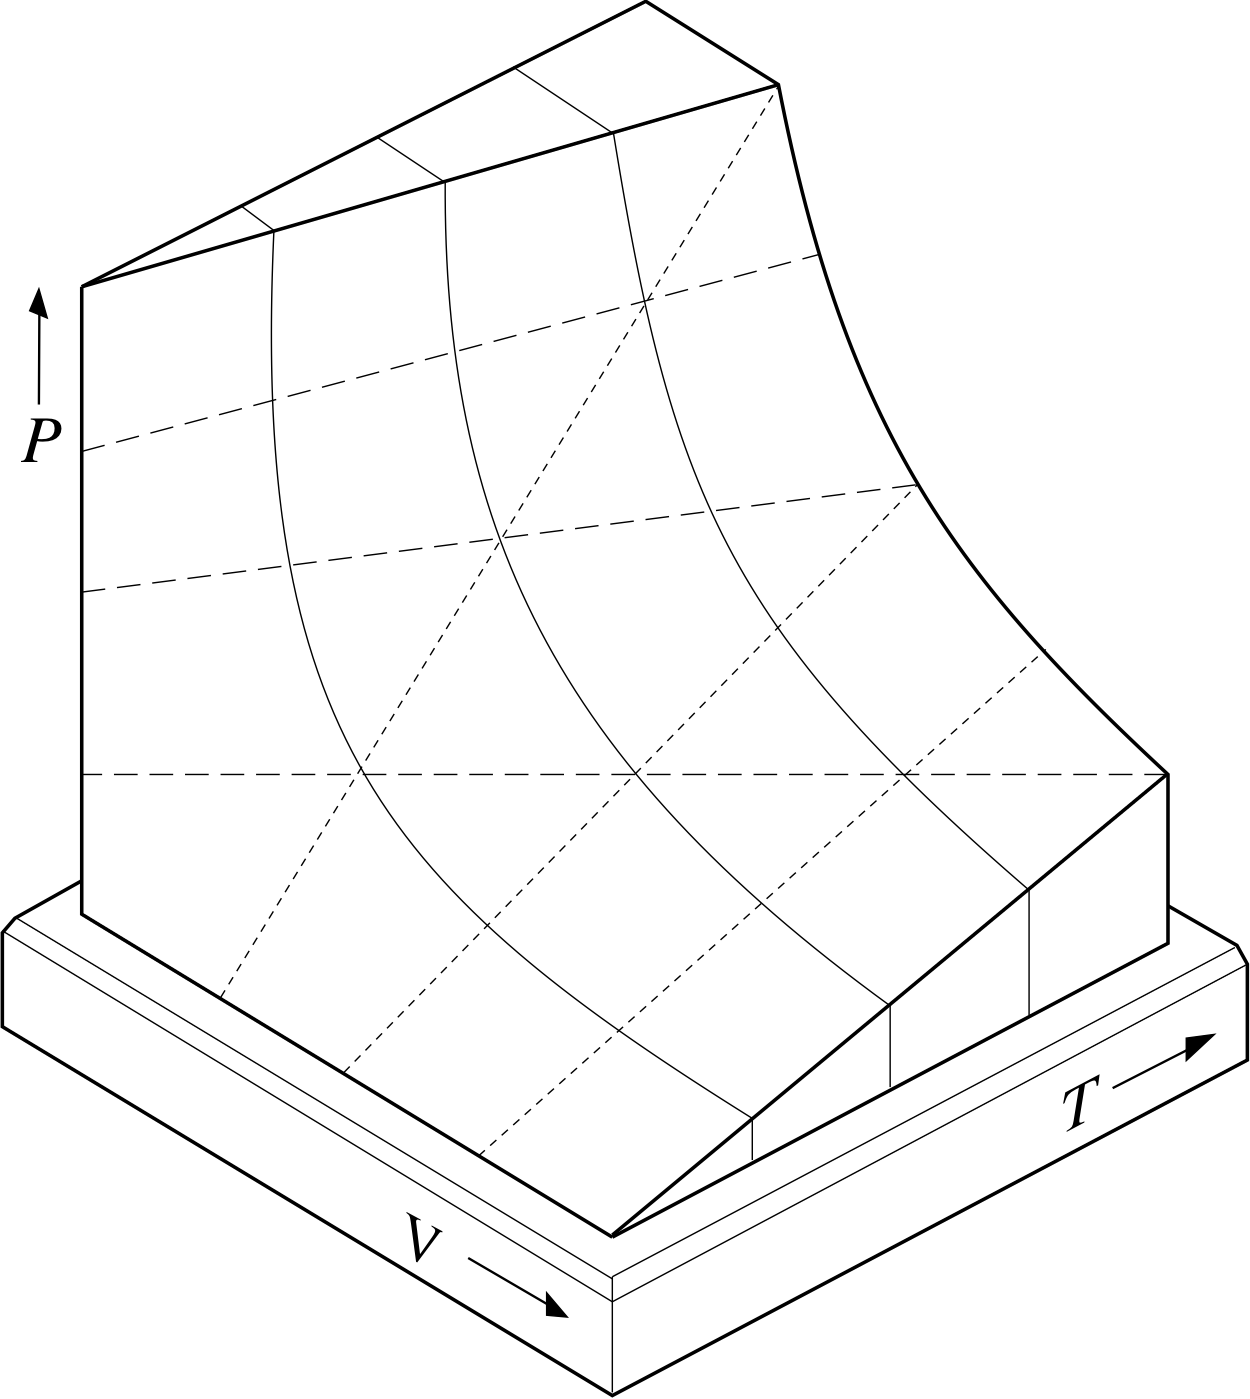
\includegraphics[keepaspectratio,width=4.3cm]{pVTgas.png}
	\caption*{PVT diagram pro ideální plyn. Body na povrchu diagramu reprezentují stavy, které může plyn nabývat}
\end{figure}

\end{columns}
}

\section{Boyleův zákon}
\frame{
   \frametitle{}
  \begin{columns}
\column{.5\textwidth}
\begin{itemize}
  \item Součin tlaku a objemu plynu je konstantní
  \item Platí pouze pro izotermické děje
  \item Není závislý na druhu plynu
  \item p.V = konst.
  \item $p_1.V_1 = p_2.V_2$
\end{itemize}

\column{.5\textwidth}
\begin{figure}
	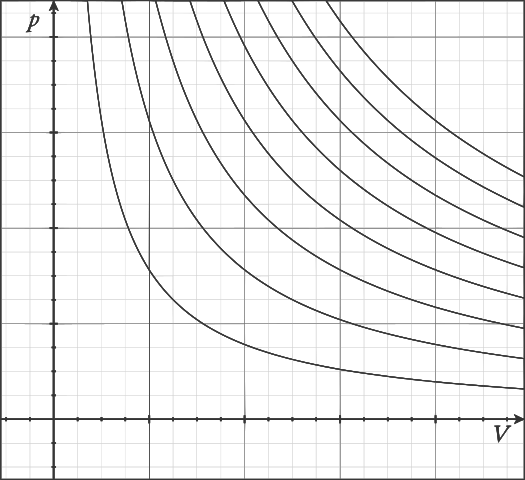
\includegraphics[width=.85\textwidth]{isotherms.png}
	\caption*{pV izotermy ideálního plynu}
\end{figure}
\end{columns}
}

\section{Daltonův zákon}
\frame{
 \frametitle{}
  \vfill
\begin{itemize}
  \item Celkový tlak směsi plynů je roven součtu parciálních tlaků všech složek směsi
  \item $p_{celk} = \sum\limits_{i=0}^n p_i$
\end{itemize}
\textbf{Parciální tlak}
\begin{itemize}
  \item Tlak komponenty ve směsi
  \item Složky směsi ideálního plynu se v nádobě chovají, jako by tam byly samy
 \item Molární zlomek
  \item \scalebox{1.3}{$X_i = \frac{n_i}{\sum n_i}$}
\end{itemize}
  \vfill
}

\end{document}